\documentclass{beamer}
\usepackage[english]{babel}
\usepackage{graphicx}
\usepackage{hyperref}

\setbeamertemplate{navigation symbols}{}

\title[PL3GA Visualisation]{Visualization of the projective geometry for geometric algebra}
\subtitle{Final Presentation}
\author{Patrick de Kok}
\institute{Supervisor: Leo Dorst}
\date{June 28, 2012}

% Math type specifying fonts
\newcommand{\V}[1]{\ensuremath{\mathbf{#1}}}
\newcommand{\s}[1]{\ensuremath{\mathcal{#1}}}

% GA operators
\newcommand{\gp}{\ensuremath{\;}}
\newcommand{\gpi}{\ensuremath{\mathbin{/}}}
\newcommand{\lcont}{\ensuremath{\mathbin{\rfloor}}}
\newcommand{\rcont}{\ensuremath{\mathbin{\lfloor}}}
\newcommand{\dotp}{\ensuremath{\mathbin{\cdot}}}
\newcommand{\dual}[1]{\ensuremath{#1^\ast}}
\newcommand{\undual}[1]{\ensuremath{#1^{-\ast}}}
%\newcommand{\edual}[1]{\ensuremath{#1^\bigstar}}
%\newcommand{\eundual}[1]{\ensuremath{#1^{-\bigstar}}}
\newcommand{\edotp}{\ensuremath{\dotp_\mathbb{E}}}
\newcommand{\elcont}{\ensuremath{\lcont_\mathbb{E}}}
\newcommand{\ercont}{\ensuremath{\rcont_\mathbb{E}}}
\newcommand{\edual}[1]{\ensuremath{#1 \lcont \epseudo^{-1}}}
\newcommand{\eundual}[1]{\ensuremath{#1 \lcont \epseudo}}
\newcommand{\norm}[1]{\ensuremath{\left\|#1\right\|}}
\DeclareMathOperator{\Em}{Em}
\DeclareMathOperator{\grade}{\mathtt{grade}}

% Homogeneous equality
\newcommand{\heq}{\ensuremath{\mathbin{=_{H}}}}

% Pl\"ucker notation
\newcommand{\plucker}[2]{\ensuremath{\{#1 \mathbin{;} #2\}}}
%\newcommand{\pluckerpoint}[2]{\ensuremath{(#1 \mathbin{:} #2)}}
%\newcommand{\pluckerplane}[2]{\ensuremath{[#1 \mathbin{:} #2]}}

% Math-like symbols
\newcommand{\reals}{\ensuremath{\mathbb{R}}}
\newcommand{\en}{\ensuremath{\mathbin{\mbox{and}}}}
\newcommand{\of}{\ensuremath{\mathbin{\mbox{or}}}}
\newcommand{\eql}{\ensuremath{\Leftrightarrow}}

\newcommand{\pline}{\ensuremath{\ell}}
\newcommand{\rline}{\ensuremath{\ell_o}}
\newcommand{\iline}{\ensuremath{\ell_\infty}}
\newcommand{\screw}{\ensuremath{s}}

\newcommand{\ez}{\ensuremath{e_0}}
\newcommand{\ee}{\V{e}_1}
\newcommand{\et}{\V{e}_2}
\newcommand{\ed}{\V{e}_3}
\newcommand{\eze}{e_{01}}
\newcommand{\ezt}{e_{02}}
\newcommand{\ezd}{e_{03}}
\newcommand{\etd}{e_{23}}
\newcommand{\ede}{e_{31}}
\newcommand{\eet}{e_{12}}
\newcommand{\epseudo}{\V{I}_3}
\newcommand{\hpseudo}{\ez\V{I}_3}

\newcommand{\ap}{a_{+}}
\newcommand{\am}{a_{-}}
\newcommand{\bp}{b_{+}}
\newcommand{\bm}{b_{-}}
\newcommand{\cp}{c_{+}}
\newcommand{\cm}{c_{-}}

\newcommand{\newterm}{$^\dagger$}

\newcommand{\ega}{\texttt{e3ga}}
\newcommand{\pga}{\texttt{p3ga}}
\newcommand{\cga}{\texttt{c3ga}}
\newcommand{\cbga}{\texttt{c5ga}}
\newcommand{\iga}{\texttt{i2ga}}
\newcommand{\lga}{\texttt{l3ga}}

\makeatletter
\def\figureautorefname{figure}
\def\tableautorefname{table}
\def\Autoref#1{%
  \begingroup
  \edef\reserved@a{\cpttrimspaces{#1}}%
  \ifcsndefTF{r@#1}{%
    \xaftercsname{\expandafter\testreftype\@fourthoffive}
      {r@\reserved@a}.\\{#1}%
  }{%
    \ref{#1}%
  }%
  \endgroup
}
\def\testreftype#1.#2\\#3{%
  \ifcsndefTF{#1autorefname}{%
    \def\reserved@a##1##2\@nil{%
      \uppercase{\def\ref@name{##1}}%
      \csn@edef{#1autorefname}{\ref@name##2}%
      \autoref{#3}%
    }%
    \reserved@a#1\@nil
  }{%
    \autoref{#3}%
  }%
}
\makeatother

\newcommand{\supcite}[1]{\textsuperscript{\cite{#1}}}
\newcommand{\pro}{\structure{\textbf{+}}}
\newcommand{\con}{\structure{\textbf{--}}}

\begin{document}
\begin{frame}
  \titlepage
\end{frame}

\begin{frame}{Project description}
    Extend a \alert<3>{graphical calculator} of \alert<1>{geometric algebra} to model the \alert<2>{projective geometry of lines}.

    \only<+>{
      \begin{itemize}
        \item Much like linear algebra, but has structure preserving operations
        \item Outer product $\wedge$ to create subspaces
        \item Implementations are fast~\supcite{Fontijne2003}
      \end{itemize}
    }
    \only<+>{
      \begin{itemize}
        \item Useful for computer vision, graphics, robotics\ldots
        \item Pl\"ucker coordinates: 3D lines are 6D null vectors
          \begin{itemize}
            \item Representation is homogeneous
          \end{itemize}
        \item Recently found an operational model for geometric algebra~\supcite{Hongbo}
      \end{itemize}
    }
    \only<+>{
      \begin{center}
        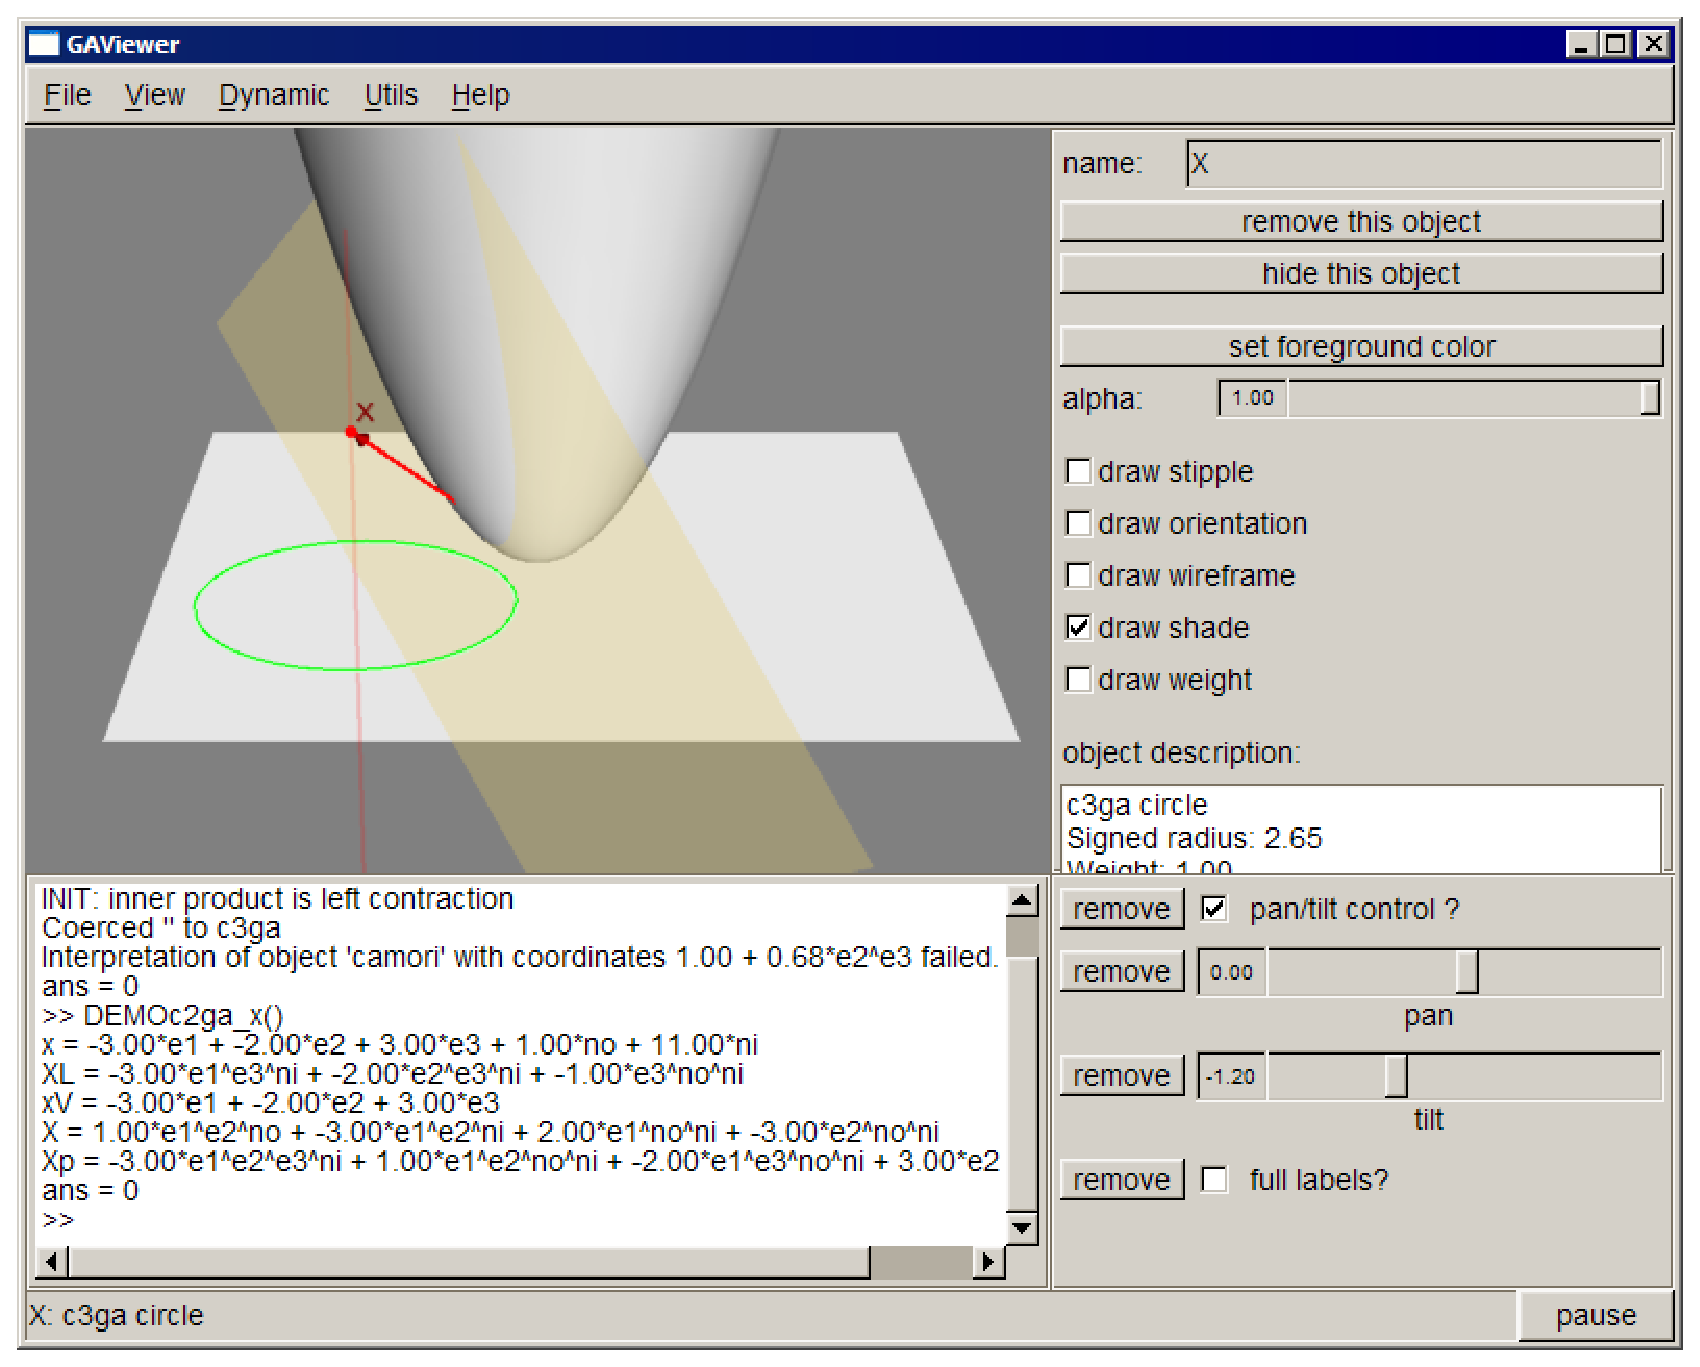
\includegraphics[width=0.7\textwidth]{gaviewer}

        \href{http://geometricalgebra.net/gaviewer_download.net}{\texttt{http://geometricalgebra.net} $\to$ Downloads $\to$ GAViewer}
      \end{center}
    }
\end{frame}

\begin{frame}{Approach}
  \begin{enumerate}
    \item Understand Pl\"ucker model for GA
    \item Explore part of the representation space
      \begin{itemize}
        \item Geometric interpretation of subspaces
        \item Compute location, stance, weight, orientation
      \end{itemize}
    \item Extend GAViewer
      \begin{itemize}
        \item Recognise geometric type of input
        \item Implement drawing routines
      \end{itemize}
  \end{enumerate}
\end{frame}

\begin{frame}{Pl\"ucker model}
  Really new to GA community
  \begin{itemize}
    \item Original article defines metric and vector space $\mathbb{R}^{3,3}$
    \item No further connection with model in other algebras shown
    \item No further articles on Pl\"ucker model for GA
  \end{itemize}
  \bigskip 
  \ldots but well known for other algebras
  \begin{itemize}
    \item Big difference in vocabulary
    \item Less focus on subspace nature
    \item Some GA concepts not well defined in LA
  \end{itemize}
\end{frame}

\begin{frame}{But first\ldots}
  Recall homogeneous model
  \begin{itemize}
    \item Extends Euclidean directions $\ee, \et, \ed$ with point $\ez$
    \item Point $p = \V{p} + \lambda \ez$ has location $\frac{p}{\ez \dotp p}$ and weight $\lambda$
    \item Directions have weight $\lambda = 0$, so location is at infinity
    \item Average of two points gives new point
  \end{itemize}
\end{frame}

\begin{frame}{Lines defined}
  \begin{columns}
    \begin{column}{5cm}
      Define line $L$ by a point $p$ and direction $\V{d}$:
      \begin{equation*}
        L  = p \wedge \V{d}
      \end{equation*}
      $\lambda L$ only differs in weight and orientation
    \end{column}
    \begin{column}{5cm}
      \begin{center}
        \includegraphics[width=5cm]{line}
      \end{center}
    \end{column}
  \end{columns}
\end{frame}

\begin{frame}{Pl\"ucker space}
  \begin{columns}
    \begin{column}{5cm}
      Basis of our vector space $\reals^{3,3}$: 
      \begin{equation*}
        \begin{array}{l}
          \left. \begin{array}{l}
            \ez\wedge\ee = \eze \\
            \ez\wedge\et = \ezt \\
            \ez\wedge\ed = \ezd
          \end{array} \right\} \mbox{Finite lines}
          \\
          \left. \begin{array}{l}
            \et\wedge\ed = \etd \\
            \ed\wedge\ee = \ede \\
            \ee\wedge\et = \eet
          \end{array} \right\} \mbox{Lines at infinity}
        \end{array}
      \end{equation*}
      %With dot product:
      %\begin{equation*}
      %  \eze \dotp \etd = \ezt \dotp \ede = \ezd \dotp \eet = 1
      %\end{equation*}
    \end{column}
    \begin{column}{5cm}
      \begin{center}
        \includegraphics[width=5cm]{line}

        \includegraphics[width=3cm]{idealline}
      \end{center}
    \end{column}
  \end{columns}
\end{frame}

\begin{frame}{Lines are screws}
  \begin{columns}
    \begin{column}{7cm}
      Screws are general basic geometric entity
      \begin{itemize}
        \item Finite lines only rotate
        \item Lines at infinity only translate
      \end{itemize}
      \ldots but we only look at subspaces of lines
    \end{column}
    \begin{column}{3cm}
      \begin{center}
        \includegraphics[width=3cm]{screw}
      \end{center}
    \end{column}
  \end{columns}
\end{frame}

\begin{frame}{Combining lines}
  Geometrical different cases
  \begin{enumerate}
    \item 2 intersecting and parallel lines
    \item 2 skew lines
    \item 3 lines intersect in 1 point
    \item 3 lines intersect in different points
    \item 1 line intersects 2 other lines
    \item 3 skew lines
  \end{enumerate}
\end{frame}

\begin{frame}{Pencils of lines}
  \begin{columns}
    \begin{column}{5cm}
      Two lines $\ell_1, \ell_2$ intersect

      \bigskip

      Parallel lines intersect in point at infinity!
    \end{column}
    \begin{column}{5cm}
      \begin{center}
      \includegraphics[width=5cm]{pencil1}

      \includegraphics[width=5cm]{pencil2}

      \includegraphics[width=5cm]{pencil3}
    \end{center}
    \end{column}
  \end{columns}
\end{frame}

\begin{frame}{Line pair}
  \begin{columns}
    \begin{column}{5cm}
      When $\ell_1, \ell_2$ don't intersect, $\ell_1 \wedge \ell_2$ only contains those two lines

      \bigskip

      Dual of $\ell_1 \wedge \ell_2$ contains all lines intersecting both 
    \end{column}
    \begin{column}{5cm}
      \begin{center}
        \includegraphics[width=5cm]{linepair1}

        \includegraphics[width=5cm]{linepair2}

        \includegraphics[width=5cm]{linepair3}
      \end{center}
    \end{column}
  \end{columns}
\end{frame}

\begin{frame}{Finite and infinite points}
  \begin{columns}
    \begin{column}{5cm}
      Two interpretations:
      \begin{enumerate}
        \item All lines intersecting in a point
        \item The point of intersection
      \end{enumerate}

      \bigskip

      Three parallel lines intersect in a pair of points
    \end{column}
    \begin{column}{5cm}
      \begin{center}
        \includegraphics[width=5cm]{point1}

        \includegraphics[width=5cm]{point2}
      \end{center}
    \end{column}
  \end{columns}
\end{frame}

\begin{frame}{Planes}
  \begin{columns}
    \begin{column}{5cm}
      If 3 lines intersect in 3 points, the linear combination is their common plane
      \bigskip
      Only 1 infinite plane, corresponds to Euclidean space
    \end{column}
    \begin{column}{5cm}
      \begin{center}
        \includegraphics[width=5cm]{plane1}

        \includegraphics[width=5cm]{plane2}
      \end{center}
    \end{column}
  \end{columns}
\end{frame}

\begin{frame}{Pair of pencils}
  \begin{columns}
    \begin{column}{5cm}
      Combines the set of lines of $\ell_1 \wedge \ell_2$, $\ell_2 \wedge \ell_3$ and $\ell_3 \wedge \ell_1$
    \end{column}
    \begin{column}{5cm}
      \begin{center}
        \includegraphics[width=5cm]{cwpencil}
      \end{center}
    \end{column}
  \end{columns}
\end{frame}

\begin{frame}{Regulus}
  \begin{columns}
    \begin{column}{5cm}
      Three skew lines

      \bigskip

      Not implemented; unclear how to parameterize the set of lines
    \end{column}
    \begin{column}{5cm}
      \begin{center}
        \includegraphics[width=5cm]{regulus1}

        \includegraphics[width=5cm]{regulus2}
      \end{center}
    \end{column}
  \end{columns}
\end{frame}

\begin{frame}{Extending GAViewer}
  Easily done:
  \begin{itemize}
    \item Generate GA code for Pl\"ucker model
    \item Only need to implement classification, visualization, what to do on mouse drag
  \end{itemize}
  
  \ldots if you know how.
  \begin{itemize}
    \item Little documentation on where to put new code
  \end{itemize}
\end{frame}

\begin{frame}{Results}
  Much is done
  \begin{enumerate}
    \item Show correspondencies between Pl\"ucker model for LA and GA
    \item Computed 4 geometrically important features of almost all line-subspaces
    \item Implemented classifications and visualizations
  \end{enumerate}
  But much more can be done
  \begin{enumerate}
    \item Compute features of reguli
    \item Compute combinations of screws
    \item Connections with other models?
    \item Ellipse representation?
    \item Pl\"ucker model for $\reals^2$?
  \end{enumerate}
\end{frame}

\begin{frame}{Questions}
  \begin{center}
    %{\Large\structure{Questions}}
    \includegraphics[width=1\textwidth]{gaviewer3}
  \end{center}
\end{frame}

\begin{frame}{Bibliography}
  \bibliographystyle{plainnat}
  \bibliography{../thesis/citations}
\end{frame}

\end{document}
